\section{Modeling and Analysis of Master Algorithm}
\label{sec:ma}
The MA provides the orchestration of FMUs, which denotes the co-simulation of various FMUs. To ensure the correctness of co-simulation, it is necessary to verify certain properties of the MA. In this section, we model three versions of MAs with TA and verify some expected properties of MAs such as deadlock, livelock and reachability with UPPAAL.
\subsection{I/O Dependency Information}
When it comes to co-simulation, I/O dependency information \cite{BromanBGLMTW13} is inevitably required to be well considered. The MA calls function \emph{Set} to provide input value to an FMU and function \emph{Get} to obtain an output value. It is of vital importance to know the dependence between input and output of FMUs. In the design of a MA, the direct dependency information can be used to call the function \emph{Set} and \emph{Get} in a well-defined order. In FMI 2.0, this information can be provided using the element \emph{ModelStructure} \cite{FMI2INTRO}. However, sometime there may be an algebraic loop in the sequence of function call, which may not converge. In section \ref{sec:sysml}, we presents water tank system to detect algebraic loop in the architecture.
\subsection{Master Algorithm}
The MA is used to orchestrate the execution of different subsystems. Each subsystem serves as an FMU component whose simulation is triggered by a particular MA. FMUs can be seen as black boxes which can be simulated independently until it needs to exchange data or synchronize. There are three versions of MAs, which are shown in Fig.~\ref{ad-fixedstep}.
\begin{figure}[htbp]
\centering{
		\subfigure[Fix step size algorithm]{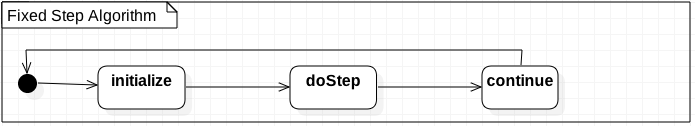
\includegraphics[width=3.5in,height=0.8in]{fig/MA1.png}
			\label{sd_fixedstep}}
		\hfil
		\subfigure[Rollback algorithm]{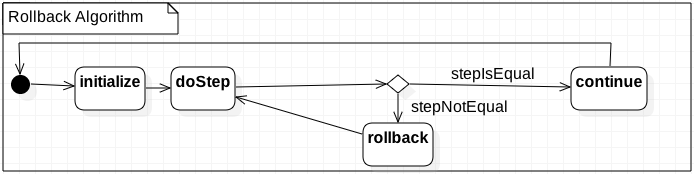
\includegraphics[width=3.5in,height=0.9in]{fig/MA2.png}
			\label{sd-rollback}}	
		\subfigure[Predictable step sizes algorithm]{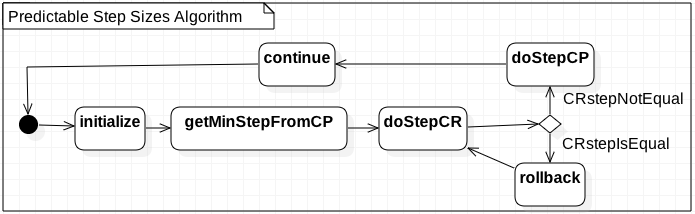
\includegraphics[width=3.5in,height=1.1in]{fig/MA3.png}
			\label{sd-pre}}		
	\caption{Activity diagrams for three versions of master algorithms.}
	\label{ad-fixedstep}
	}
\end{figure}
\subsubsection{Fixed Step Algorithm}
For fixed step algorithm, all FMUs have the same step size. When MA calls \emph{doStep} with the step size \emph{h}, it will advance from a communication point \emph{t} to the next communication point \emph{t+h}. During the simulation step, an FMU with its own solver will simulate independently according to its input value and generate a running result as output value. MA will wait until all FMUs finish their simulation step and then get their output values to exchange data for preparing the next simulation step. The activity diagram for fixed step algorithm is illustrated in Fig.\ref{sd_fixedstep}. There are mainly three activities in the control flow: \emph{initialize}, \emph{doStep} and \emph{continue}. In the fixed step algorithm \cite{BromanBGLMTW13}, the co-simulation process should be reliable, when all FMUs are reliable. When some error happens during a simulation step, the co-simulation will be affected due to the wrong simulation step. To overcome the shortcoming of the fixed step algorithm, it needs rollback mechanism.
\subsubsection{Rollback Algorithm}
There are some important features proposed in the FMI 2.0. It supports to save the FMU state if necessary and the saved state can be restored. For example, MA calls \emph{doStep} on $FMU_{1}$ and $FMU_{2}$ while $FMU_{1}$ can accept the request or $FMU_{2}$ can reject it. If we save the state of $FMU_{1}$ and $FMU_{2}$ at the communication point, we can restore the scene after $FMU_{2}$ rejects \emph{doStep}. The activity diagram of rollback algorithm \cite{BromanBGLMTW13} is clearly shown in Fig.\ref{sd-rollback}. Compared with the fixed step algorithm, all FMUs are required to support \emph{rollback} mechanism, that is, all FMUs could return to the previous state if the step sizes of all FMUs simulation are not equal.
\subsubsection{Predictable Step Size Algorithm}
To improve the efficiency of MA, it is important to predict the step size. So, predictable step size algorithm is proposed \cite{BromanBGLMTW13}. The function \emph{GetMaxStepSize} was introduced to optimize the performance of rollback algorithm. This function returns the maximum step size and state flag of a predictable FMU. Maximum step is the largest step that a predictable FMU can perform. State flag includes \emph{ok}, \emph{discard} and \emph{error}. \emph{OK} denotes the predictable FMU can accept the simulation step size. \emph{Discard} denotes the predictable FMU only implement partial step during simulation. \emph{Error} denotes the predictable FMU can't continue the simulation because of its unacceptable state or unreasonable input value. When \emph{discard} and \emph{error} occur, the FMU needs to rollback to the previous saved state. Whether an FMU is predictable or not, it should be indicated in FMU's \emph{xml} file. Moreover, if an FMU supports rollback and predictable step size at the same time, the predictable step size algorithm can get the maximum step size of the FMU using \emph{GetMaxStepSize} function.

In predictable step size algorithm, MA chooses the maximum step size of all predictable FMUs and find the smallest communication step size \emph{h} which ensure all predictable step size can be accepted. Then, the states of all FMUs are saved. MA calls \emph{doStep(h)} function of FMUs which support rollback. The function \emph{doStep()} will return the real performed step size. If all performed step sizes are equal to \emph{h}, MA will call \emph{doStep(h)} for FMUs. Otherwise, MA will find the smallest performed step $h_{min}$, then all FMUs will restore the saved state. Finally, MA will invoke $doStep$ $(h_{min})$ on all FMUs. The control flow of predictable step size algorithm is shown in Fig.\ref{sd-pre}. For example, \emph{getMinStepFromCP} is an activity that MA will call \emph{GetMaxStepSize} on all predictable FMUs to find their maximum simulation step size and then choose the smallest one of them. 

\subsection{Modeling and Verification of MA} 
UPPAAL is a toolset for verification of real-time systems represented by (a network of) TA which is extended with integer variables, structured data types, and channel synchronization. We model the TAs using TA in UPPAAL. The Fig.\ref{ta-master} shows the TA models of three MAssssss,  respectively. Fixed step algorithm has \emph{Init}, \emph{doStep} states and synchronize with \emph{FMU} by channel \emph{continue}. Rollback algorithm has \emph{Init}, \emph{DoStep}, and \emph{Continue} states. If all FMUs don't have the same step size, rollback algorithm will communicate with FMUs by \emph{rollback} signal, otherwise, it will send \emph{continue} signal and move to \emph{Continue} state. Predictable step size algorithm has \emph{Init}, $find \_ CP \_ MIN$, \emph{DoStep}, \emph{writeCP} states. It obtains the minimal step size (i.e., \emph{step2}) of FMUs supporting \emph{GetMaxStepSize} function and the maximal step size (i.e., \emph{step1}) of FMUs supporting rollback. If \emph{step1} is greater than \emph{step2}, FMUs receive \emph{rollback} signal and return to \emph{DoStep} state. Otherwise, FMUs receive \emph{continue} signal and do next step.  

\begin{figure}[htbp]
\centering{
		\subfigure[TA for fixed step algorithm]{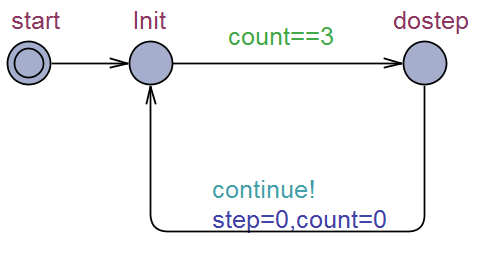
\includegraphics[width=1.0in,height=0.8in]{fig/fixedstep_master.png}
			\label{ta_fixedstep}}
		\hfil
		\subfigure[TA for rollback algorithm]{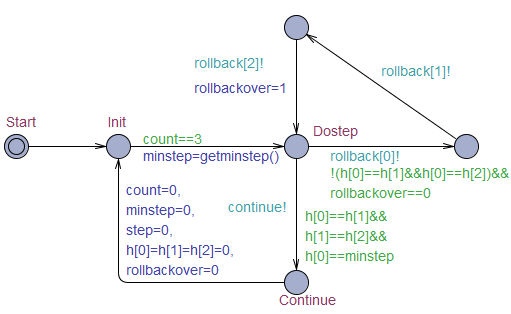
\includegraphics[width=2.0in,height=1.2in]{fig/rollback_master.png}
			\label{ta-rollback}}	
		\subfigure[TA for predictable step size algorithm]{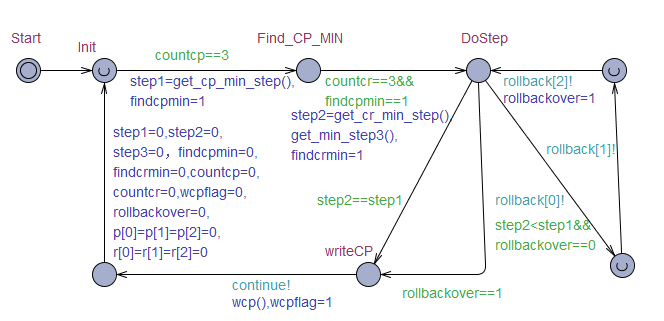
\includegraphics[width=3.5in,height=1.6in]{fig/pma_master.png}
			\label{ta-pre}}		
	\caption{TA for three versions of MAs.}
	\label{ta-master}
	}
\end{figure}

We verify the properties of three various MAs including reachability, liveness and deadlock. Experimental results are shown in Table \ref{ta_r}.

\begin{itemize}
\item
$E \langle\rangle ~master.dostep$, $E\langle\rangle~master.Continue$ and $E\langle\rangle~master.writeCP$ are reachability properties checking whether the model can reach these states;
\item
$master.Init \rightarrow master.dostep$, $master.Init \rightarrow master.Continue$ and $master.Init \rightarrow master.Continue$ are liveness properties. If the MA arrives at the former state, it eventually reaches the latter state;
\item
$A[]~not~deadlock$ is safety property, which means whether the model will be deadlock.
\end{itemize}

Table \ref{ta_r} shows that the properties such as deadlock, liveness and reachability are satisfied, which ensures that the correctness of MA. For example, The property $A[]~not~deadlock$ is satisfied, which means the MA is deadlock free. The property $master.Init \rightarrow master.doStep$ is satisfied, which means if the model reach the former state $Init$, it will eventually reach the state $doStep$. The property $E\langle\rangle~master.doStep$ is satisfied, which means there exists a reachable state $doStep$. 

\begin{table}
\caption{Experimental results for verifying MA}
\centering
\begin{tabular}{c c c}
        \hline
        MA & Property & Result\\
        \hline
        \multirow{2}{2.0cm}{Fixed Step}
                & $A[]~not~deadlock$ & True\\
                & $master.Init \rightarrow master.dostep$ & True\\
                & $E\langle\rangle~master.dostep$ & True\\

        \hline
        \multirow{2}{2.0cm}{Rollback}
                & $A[]~not~deadlock$ & True\\
                & $master.Init \rightarrow master.Continue$ & True\\
                & $E\langle\rangle~master.Continue$ & True\\

        \hline
        \multirow{2}{2.0cm}{Predictable}
                & $A[]~not~deadlock$ & True\\
                & $master.Init \rightarrow  master.writeCP$ & True\\
                & $E\langle\rangle~master.writeCP$ & True\\
        \hline
\end{tabular}
\label{ta_r}
\end{table}

